%
% Chapter 3 - Results
%
\chapter{Results}

This chapter shows what has been achieved and developed to this date.\\

As previously written in the project's roadmap, this project has already a working relational database
and a HTTP server, developed with postgreSQL and with kotlin and spring mvc, respectively. The group also
managed to achieve, as planned, its first working plaform client - a prototype android mobile application, developed
with kotlin.

\section{Relational database}

As a result of multiples redesigns, here is the database's final conceptual model.

\begin{figure}[H]    
    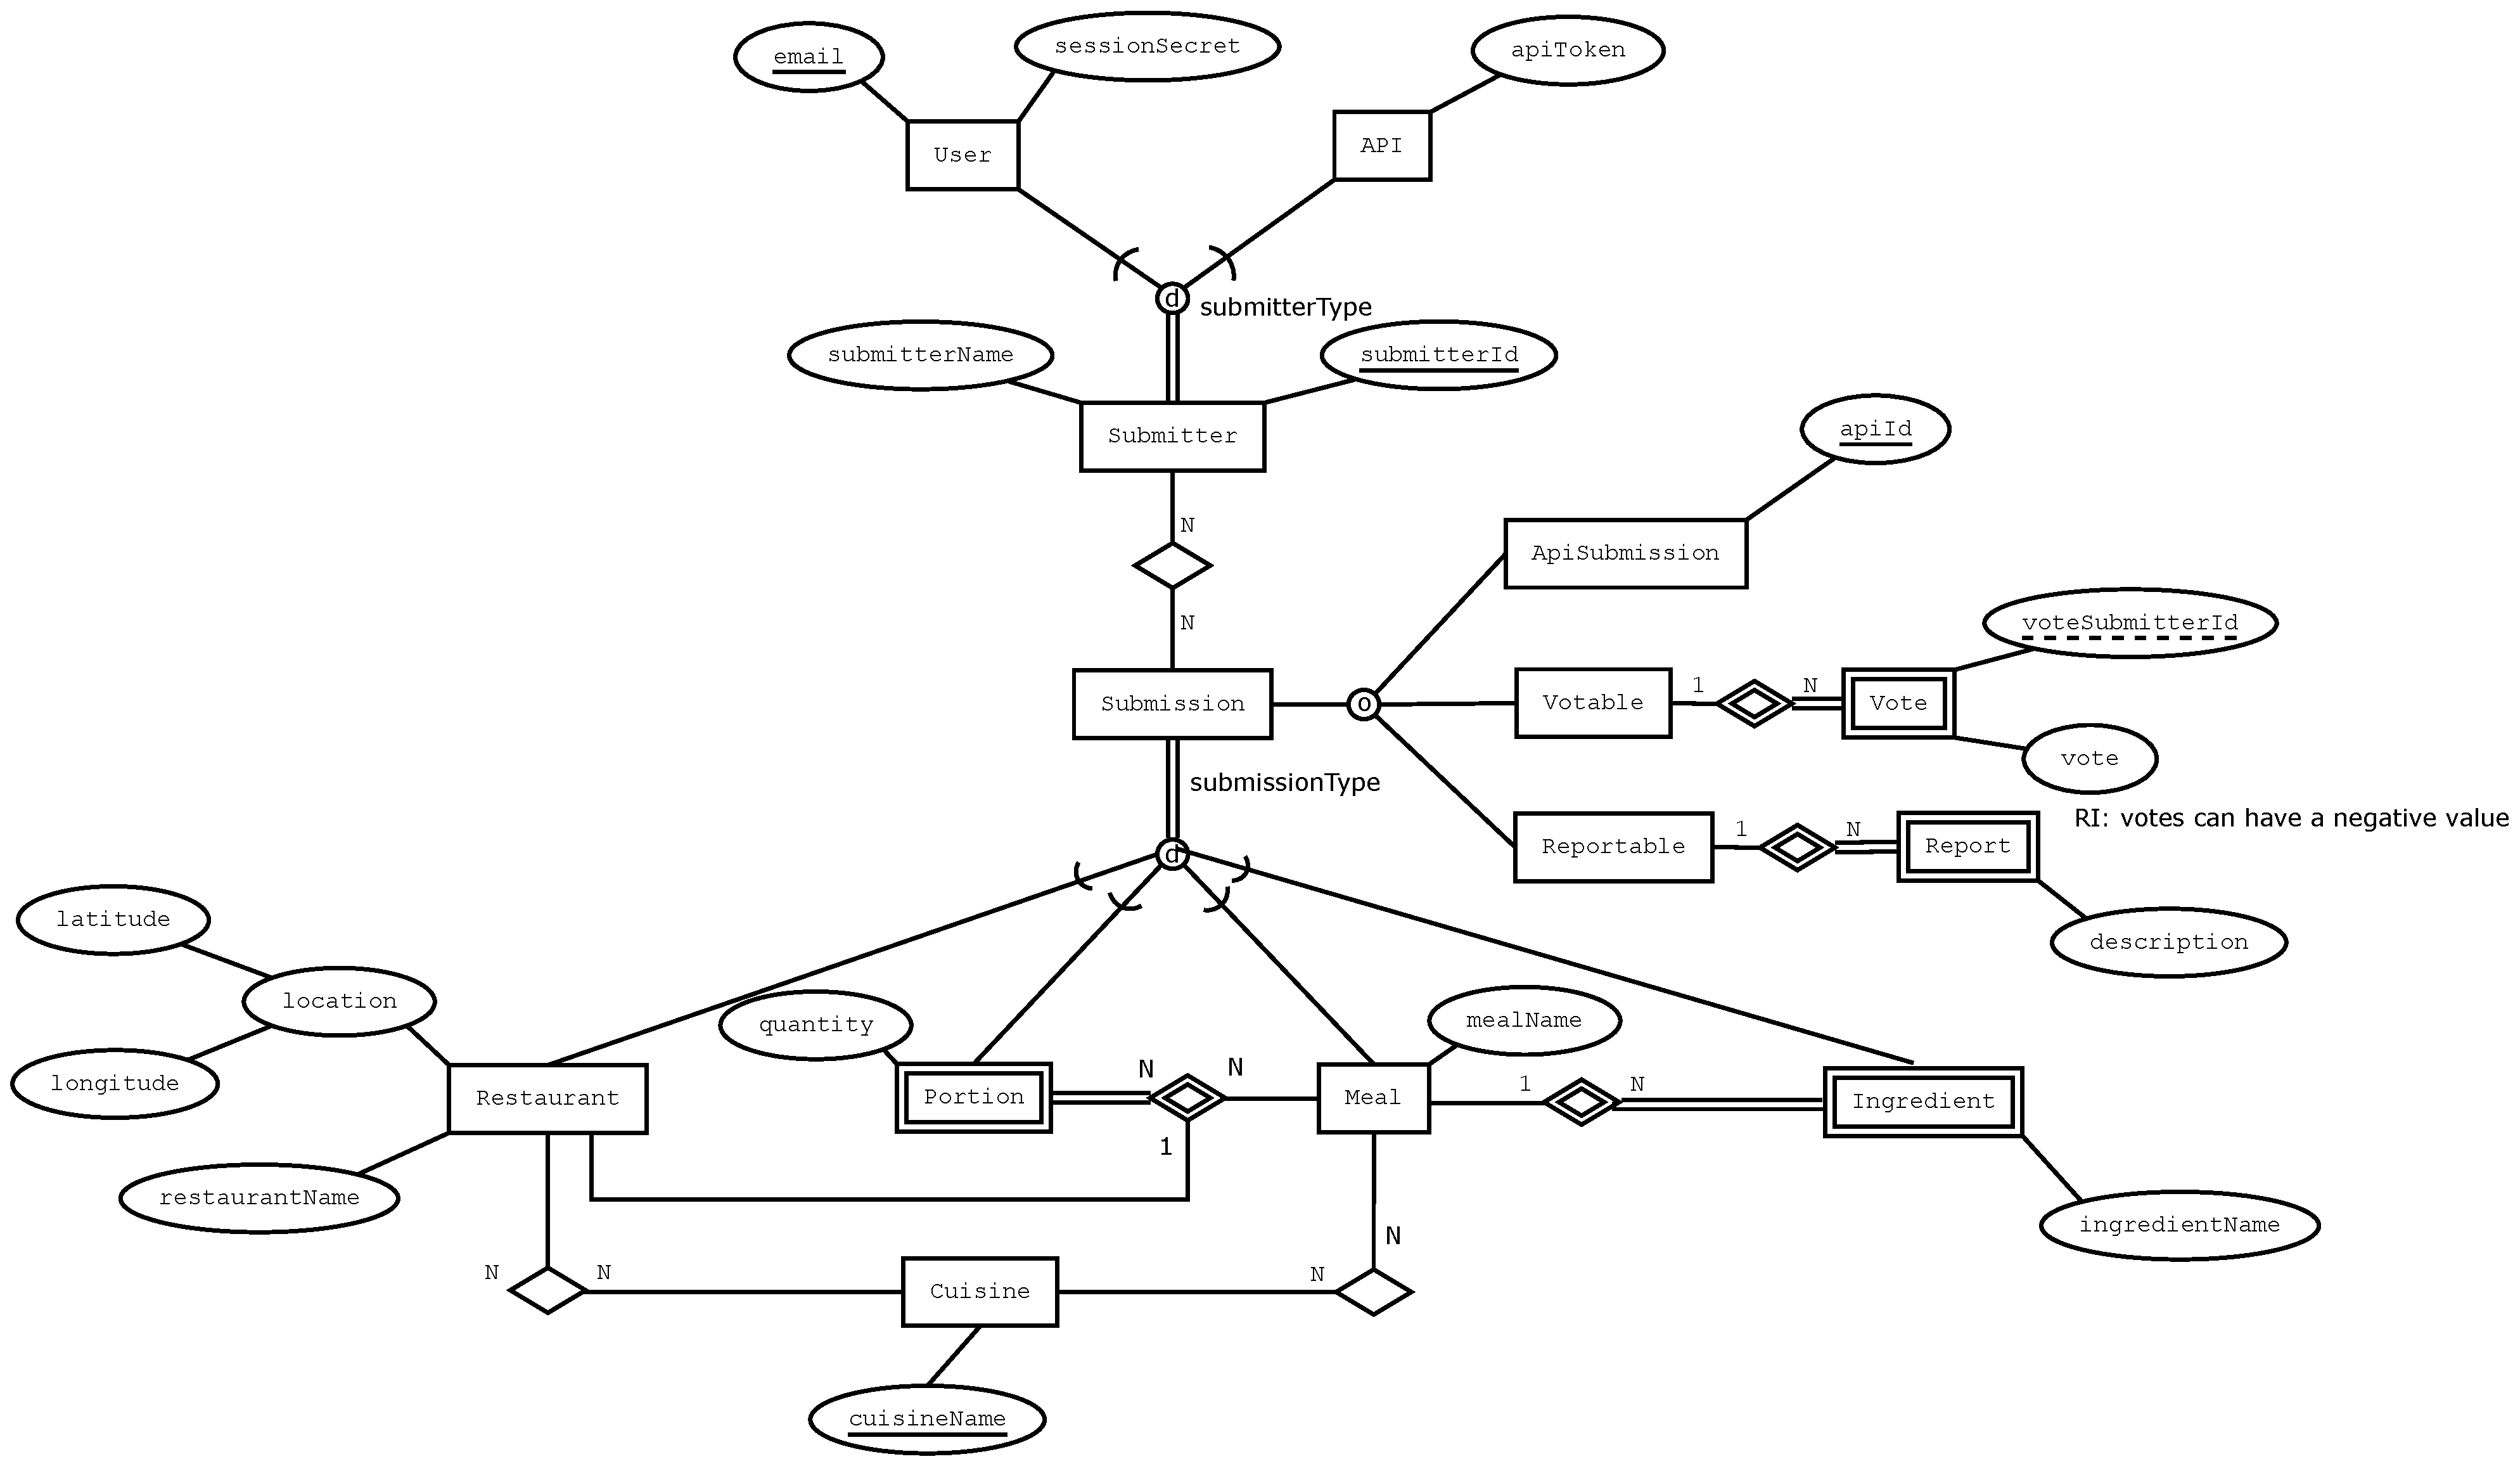
\includegraphics[scale=0.25]{_figures/Nutr.io_Database_Diagram.eps}
    \caption{Database conceptual model}
\end{figure}

\newpage
The database's relational model is present inside this report's appendix [\nameref{app:relational_model}].\\

In the relational model there are tables which are not specified in the conceptual model.
These are a product from associations between entities which will simplify queries' complexity.\\

The best feature of this redesigned model is that the database can filter user's submissions from API submissions. This is very
useful because when a user tries to associate a meal that does not exist in the database to a restaurant that is already registered
in the database, the system will need to search for that meal in an external API. When the meal is found, it will be inserted in the database
as an API submission, because the data came from an external API.\\

However if another user inserts this previously inserted meal to another registered restaurant, it will insert as an user's submission, because
the data already exists in the database and the user just built the association between the specific the meal and the specific restaurant.\\

This process, which resembles how memory pointers work, provides a high scalability and, cooperatively with the database normalization, lowers the memory usage.\\

\section{HTTP server}

The HTTP server is being developed in Kotlin and Spring MVC and during the starting phase of development the group had to define its endpoints [\nameref{app:endpoints_table}] 
and content negotiation, namely, the content type of a valid and invalid response.\\

After discussing between application/vnd.siren+json and application/json for valid responses, the group decided on application/json due to its simplicity and ease of use.
As for invalid responses, the group preferred application/problem+json over application/json, in order to avoid the need to define new error response formats.\\

\section{Geolocation}

Given how all clients rely on obtaining nearby restaurants, there was a need to implement a geolocation function in the project's design.\\

Initial research showcased two possible solutions: Haversine distances and cartesian distances, where the latter returns a highly imprecise distances.
As such, Haversine was selected.\\

The next step was to choose which system filters nearby restaurants: database or HTTP server. After some discussion, the group decided that database was the best
option for two reasons: 
\begin{itemize}
    \item Given the large amount of existing restaurants, sending such data from the database to the HTTP server so that it could filter it would occupy too much memory;
    \item PostgreSQL already supplies extensions that add support for location queries, namely PostGIS.
\end{itemize}

\section{Android application}

Being a prototype, the mobile application has only the core features to work and interact with the HTTP server.

The group chose to create an application that offers a minimalist layout to the user, providing accessible menus and a
menu drawer, which implies the use of fragments instead of activities.\\

The following weeks will focus on implementing a map displaying fragment, which the group expects to be challenging as the group needs to learn how to use a complex framework.\\

The volley framework was implemented to allow the application to make asynchronous server requests.\\

As all of the server endpoints send responses in JSON format, the application depends on the Jackson library to deserialize and serialize this format.